\chapter{The models}
In this chapter we discuss several neural network classifiers and their results on our dataset.
\section{Baseline model}
\label{sec:baselinemodel}
We decided to start with an adaptation of the \textit{optimal} model's architecture outlined in \cite{blackardDean} and reported in Figure \ref{fig:baselinemodel}. The model is made of 51 input nodes, 120 hidden nodes and seven output nodes (symbolized as baseline-51-120-7) where each layer is fully connected. Both the hidden and output layers utilized the logistic (sigmoid) activation functions:
$$
\sigma(a) = \frac{1}{1 + e^{-a}}\text{.}
$$
The 51 input features are obtained from the 54 initial ones by using <<Distance\_To\_Hydrology>> feature as described in Section \ref{sec:feat_eng} and by dropping <<Aspect>> and <<Slope>> features since the hillshade ones, according to their definition, vary depending on a factor
\begin{equation}
\begin{aligned}
\alpha&=\cos(Slope)\cdot \cos(90-Altitude)+ \\
& +\sin(Slope) \cdot \sin(90-Altitude)\cdot \cos(Azimuth-Aspect)\text{,}
\end{aligned}
\end{equation}
that already contains the same information the dropped features carry. Given the training set size, we picked SGD (Stochastic Gradient Descent) as loss function optimizer, while the loss function is the classic MSE (Mean Squared Error, as in \cite{blackardDean}):
\begin{equation}
\text{MSE} = \frac{1}{N}\sum_{i=1}^{N}(Y_i - Y^{*}_{i})^2
\end{equation}
where $Y_i$ is the vector of the true values of the target, $Y^{*}_{i}$ is the model's prediction and $N$ is the number of samples. After running a grid-search algorithm over a set of hyperparameters, the best model was found (learning rate (LR) to $0.05$, batch size to $128$ and number of epochs to $200$): the classifier has then been trained via a 10-fold cross-validation. The accuracy on the train set and the validation set is shown in Figure \ref{fig:baselinemodelacc} while the losses in Figure \ref{fig:baselinemodelloss}: to smooth the plots, the last metric value for each fold has been taken into account.
\begin{figure}
\centering
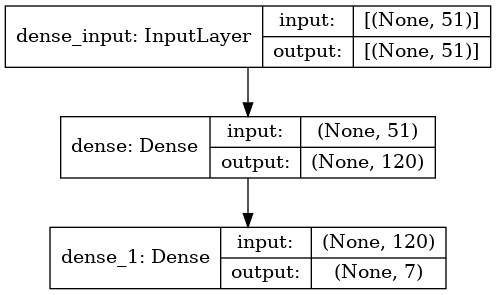
\includegraphics[width=0.7\textwidth]{./TeX_files/img/baselinemodel.png}
\caption{Baseline model diagram.}
\label{fig:baselinemodel}
\end{figure}

\begin{figure}
\centering
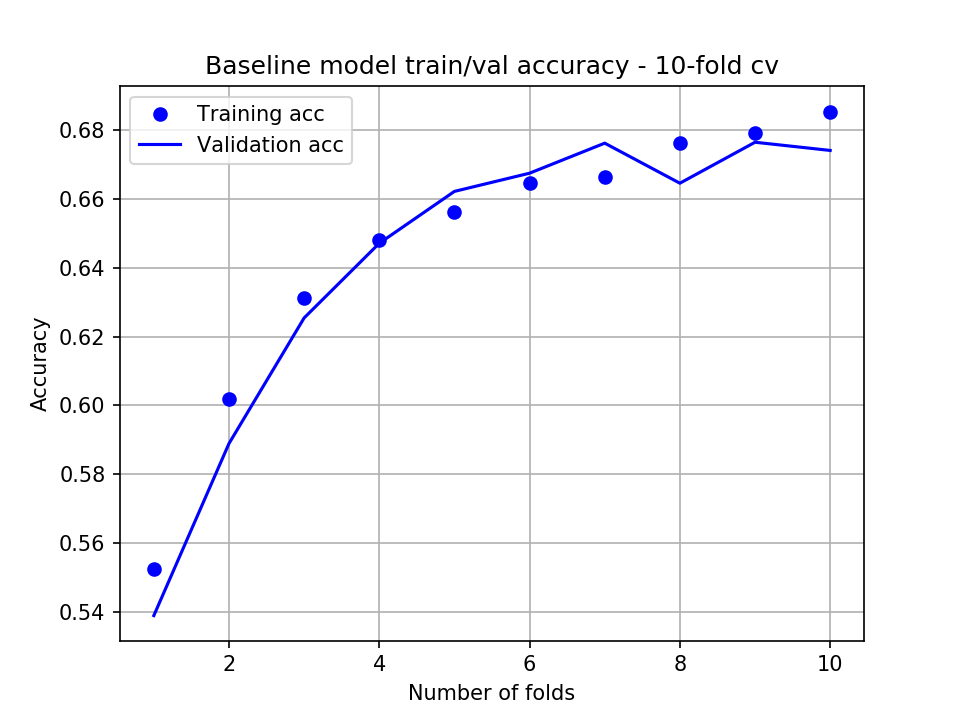
\includegraphics[width=0.7\textwidth]{./TeX_files/img/baselinemodelacc.png}
\caption{Baseline model accuracy.}
\label{fig:baselinemodelacc}
\end{figure}

\begin{figure}
\centering
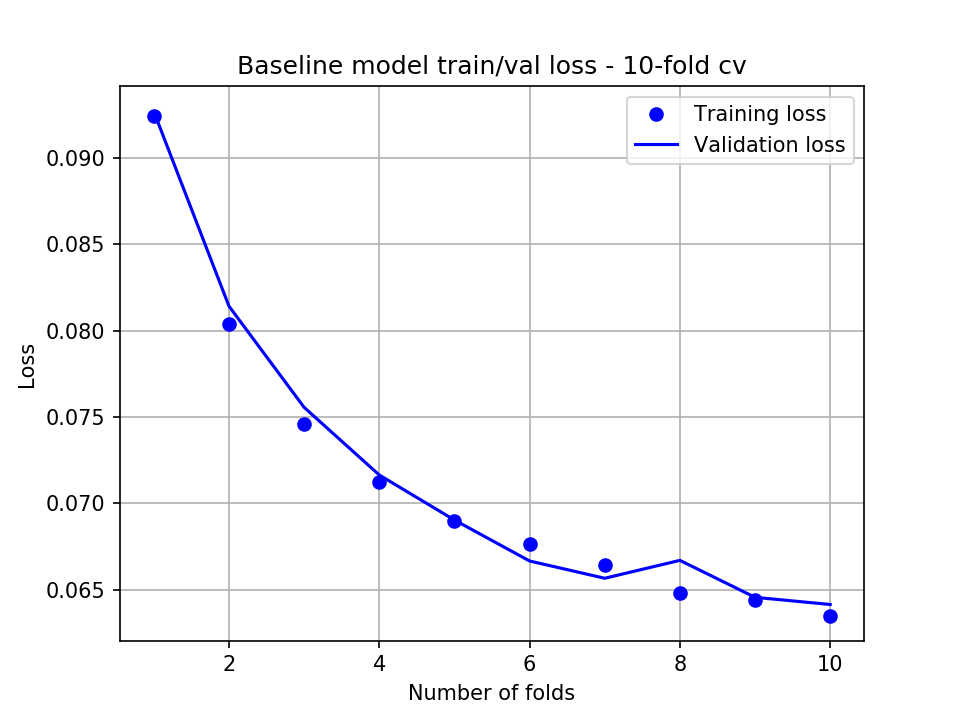
\includegraphics[width=0.7\textwidth]{./TeX_files/img/baselinemodelloss.png}
\caption{Baseline model losses.}
\label{fig:baselinemodelloss}
\end{figure}
Given the multi-class nature of the classification task, Figure \ref{fig:baselineconfmatheatmap} represent the heat-map rendering of the classification matrix to better convey the information regarding the correctly classified/misclassified samples: it is easy to notice that $532$ samples, of the total $587$ in the test set, belonging to the minority class (Cottonwood/Willow) are correctly classified; $5285$ are misclassified as the minority class but they belong to Ponderosa Pine. Moreover, a good amount of Spruce/Fir samples are correctly classified (this should be expected since this class is one of the majority classes). Other useful performance metrics for imbalanced class problems are precision (PRE), recall (REC) and F1-score (F1):
\begin{equation}
\begin{aligned}
\text{PRE} &= \frac{TP}{TP+FP}\text{,} \\
\text{REC} &= \frac{TP}{FN+TP}\text{,} \\
\text{F1} &= 2 \cdot \frac{\text{PRE} \cdot \text{REC}}{\text{PRE} + \text{REC}}\text{,}
\end{aligned}
\end{equation}
where $TP$ stands for True Positive, $FP$ for False Positive and $FN$ for False Negative. According to these definitions, Table \ref{tab:baselineclassificationrep} summarises each metric for all $7$ classes: as expected, the first minority class Cottonwood/Willow exhibits high recall ($\sim90.63\%$) and very low precision ($\sim6.95\%$) which means that the classifier is giving a lot of positive predictions while being wrong most of the times (the classifier confuses quite often samples belonging to other classes as samples belonging to this class); the second minority class Aspen is pretty much the same, high recall ($\sim71.96\%$) and low precision ($\sim6.63\%$). For the majority class Spruce/Fir the classification looks quite reasonable (recall $\sim64.75\%$, precision $\sim66.37\%$), mainly because the class represents a huge part of the dataset. In fact, during the validation phase, the model having highest accuracy is picked and this will necessarily involve a high recall value for the aforementioned class. Finally, the weighted avg column represent a weighted average of each precision metric where the weights are the support value for each class. For example, the weighted avg of the precision column is calculated as Equation \ref{eq:weighavgprec}:
\begin{equation}
\label{eq:weighavgprec}
\begin{aligned}
&\frac{(209679)0.6637 + (281141)0.7898 + (33594)0.6497+(587)0.0695}{565892}+ \\
&+\frac{(7333)0.0663 + (15207)0.2611 + (18350)0.3569}{565892} \approx 0.6964.
\end{aligned}
\end{equation}
\begin{figure}
\centering
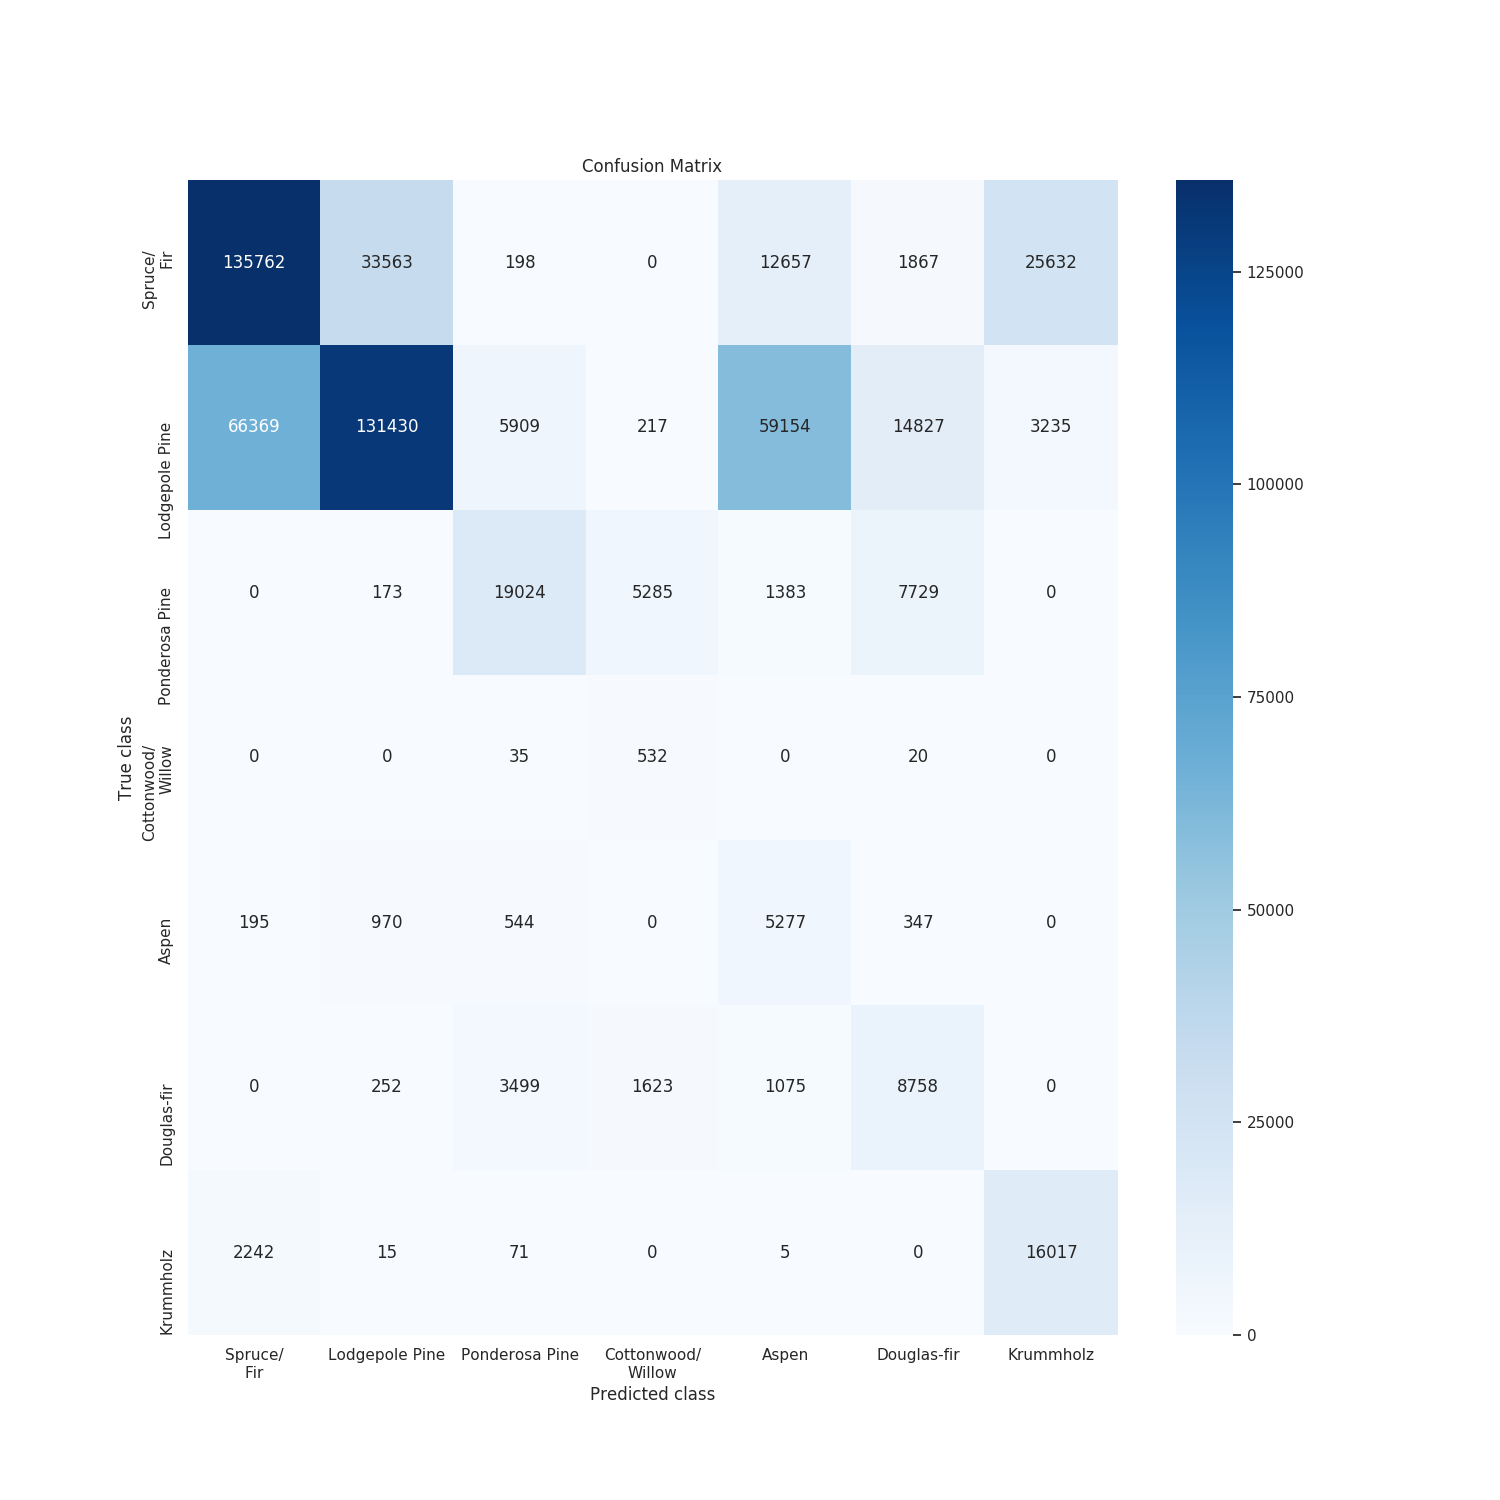
\includegraphics[width=\textwidth]{./TeX_files/img/baselineconfmatheatmap.png}
\caption{Heat-map rendering of the confusion matrix for the baseline model.}
\label{fig:baselineconfmatheatmap}
\end{figure}
% La tabella va aggiustata come in 
% https://tex.stackexchange.com/questions/2441/how-to-add-a-forced-line-break-inside-a-table-cell
\begin{table}
\centering
\resizebox{0.9\textwidth}{!}{
\begin{tabular}{ccccc}
& precision & recall & f1-score & support \\ \hline
Spruce/Fir        & 0.6637    & 0.6475 & 0.6555   & 209679  \\ \hline
Lodgepole Pine    & 0.7898    & 0.4675 & 0.5873   & 281142  \\ \hline
Ponderosa Pine    & 0.6497    & 0.5663 & 0.6051   & 33594   \\ \hline
Cottonwood/Willow & 0.0695    & 0.9063 & 0.1291   & 587     \\ \hline
Aspen             & 0.0663    & 0.7196 & 0.1215   & 7333    \\ \hline
Douglas-fir       & 0.2611    & 0.5759 & 0.3593   & 15207   \\ \hline
Krummholz         & 0.3569    & 0.8729 & 0.5066   & 18350   \\ \hline
weighted avg      & 0.6964    & 0.5598 & 0.5984   & 565892  \\ \hline
test set accuracy          & 0.5598    & 0.5598 & 0.5598   & 0.5598  \\ \hline
\end{tabular}
}
\caption{Precision, recall, f1-score summary table for the baseline model. Support indicates the number of occurrences of each particular class in the true responses (for the test set). Weighted avg is the per metric weighted average where the weights correspond to the support of that class.}
\label{tab:baselineclassificationrep}
\end{table}
\section{Proposed models}
Inspired by what we have seen so far, we tried to come up with possible good classifiers while trying to keep it simple. Section \ref{sec:onehidden} goes through a model similar to the baseline of Section \ref{sec:baselinemodel}. Section \ref{sec:twohidden} present a completely different model based on our intuition of neural networks.
\subsection{One hidden layer network}
\label{sec:onehidden}
The model is made of 51 input nodes, 120 hidden nodes and seven output nodes (symbolized as onehidden-51-120-7) where each layer is fully connected (same architecture as Figure \ref{fig:baselinemodel}). The hidden layer activation function is the ReLU:
\begin{equation}
\text{ReLU}(a) = (a)_+ = a\cdot[a>0].
\end{equation}
The output layer activation function is the softmax:
\begin{equation}
\text{Softmax}(a)_j = \frac{\exp(a_j)}{\sum_{c=1}^{C} \exp(a_c)}, \; j = 1,2,\dots,C 
\end{equation}
where $C$ is the number of classes ($C=7$ for our classification task). The loss function optimizer is again SGD and the loss function is the Cross Entropy:
\begin{equation}
\begin{aligned}
- \frac{1}{N} \sum_{i=1}^{N}\sum_{c=1}^{C} [y_i = c] \log p_{model}(y_i = c)
\end{aligned}
\end{equation}
where N is the number of samples, C the number of classes, $p_{model}(y_i = c)$ the probability, predicted by the model for the $i$-th sample, of belonging to the $c$-th class. After running a grid-search algorithm over a set of hyperparameters, the best model was found (learning rate to $0.5$, batch size to $128$ and number of epochs to $100$): the classifier has then been trained via a 10-fold cross-validation. The accuracy on the train set and the validation set is shown in Figure \ref{fig:onehiddenmodelacc} while the losses in Figure \ref{fig:onehiddenmodelloss}. It is easy to notice a slight improvement compared to the baseline. Figure \ref{fig:onehiddenconfmatheatmap} and Table \ref{tab:onehiddenclassificationrep} confirm that the learning process has improved: only $32$ over $587$ samples of Cottonwood/Willow are misclassified; $15774$ samples are classified as Aspen but they belong to Lodgepole Pine which, compared to the baseline, is an improvement of $\sim3.8$ times (namely, $15774$ against $59154$). It is quite clear that this model trains faster than the baseline and performs way better.
\begin{figure}
\centering
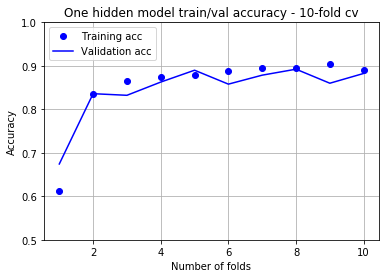
\includegraphics[width=0.7\textwidth]{./TeX_files/img/onehiddenmodelacc.png}
\caption{One hidden model accuracy.}
\label{fig:onehiddenmodelacc}
\end{figure}
\begin{figure}
\centering
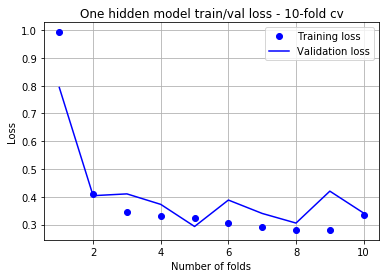
\includegraphics[width=0.7\textwidth]{./TeX_files/img/onehiddenmodelloss.png}
\caption{One hidden model losses.}
\label{fig:onehiddenmodelloss}
\end{figure}
\begin{figure}
\centering
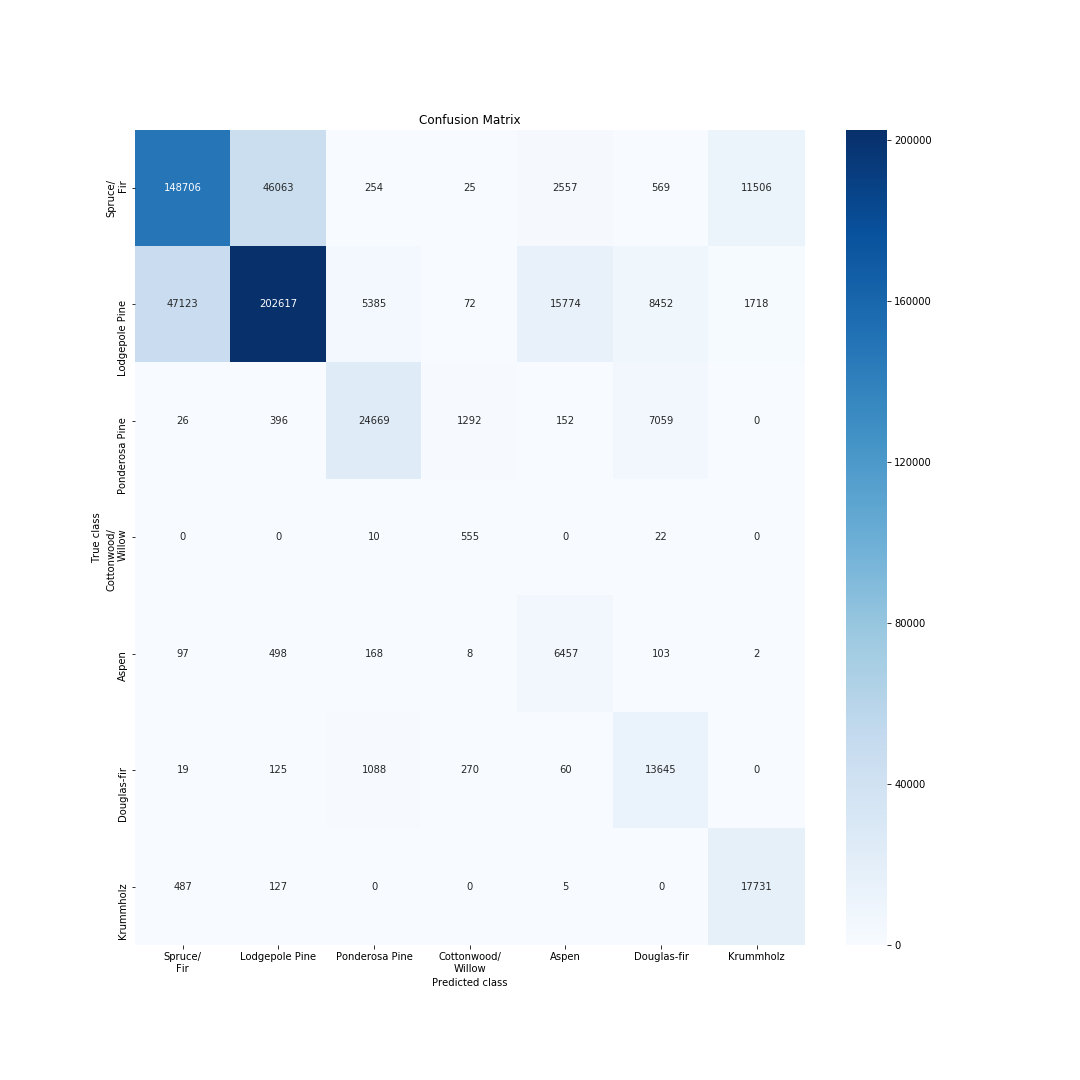
\includegraphics[width=\textwidth]{./TeX_files/img/onehiddenconfmatheatmap.png}
\caption{Heat-map rendering of the confusion matrix for the one hidden layer model.}
\label{fig:onehiddenconfmatheatmap}
\end{figure}
\begin{table}
\centering
\resizebox{0.9\textwidth}{!}{
\begin{tabular}{ccccc}
& precision & recall & f1-score & support \\ \hline
Spruce/Fir        & 0.7569    & 0.7092 & 0.7323   & 209680  \\ \hline
Lodgepole Pine    & 0.8110    & 0.7207 & 0.7632   & 281141  \\ \hline
Ponderosa Pine    & 0.7813    & 0.7343 & 0.7571   & 33594   \\ \hline
Cottonwood/Willow & 0.2498    & 0.9455 & 0.3952   & 587     \\ \hline
Aspen             & 0.2582    & 0.8805 & 0.3993   & 7333    \\ \hline
Douglas-fir       & 0.4571    & 0.8973 & 0.6057   & 15207   \\ \hline
Krummholz         & 0.5728    & 0.9663 & 0.7192   & 18350   \\ \hline
weighted avg      & 0.7642    & 0.7323 & 0.7406   & 565892  \\ \hline
test set accuracy          & 0.7323    & 0.7323 & 0.7323   & 0.7323  \\ \hline
\end{tabular}
}
\caption{Precision, recall, f1-score summary table for the one hidden layer model.}
\label{tab:onehiddenclassificationrep}
\end{table}
\subsection{Two hidden layers network}
\label{sec:twohidden}
Based on our experience with the Forest Cover Type dataset we came up with a different architecture shown in Figure \ref{fig:twohiddenmodel}. This model consists of 51 input nodes, 2 hidden layers (the first one made of 30 nodes while the second one of 15 nodes) and seven nodes for the output layer; each layer is fully connected, as usual. Both hidden layers activation functions are ReLU and the output layer is, again, the softmax. The loss function optimizer and the loss function are equal to the one hidden layer model.
After running a grid-search algorithm over a set of hyperparameters, the best model was found (learning rate to $0.3$, batch size to $128$ and number of epochs to $100$): the classifier has then been trained via a 10-fold cross-validation. The accuracy on the train set and the validation set is shown in Figure \ref{fig:twohiddenmodelacc} while the losses in Figure \ref{fig:twohiddenmodelloss}. Even though the network performs slightly worse than onehidden-51-120-7, it has $2085$ edges (vs $6960$) thus the computational burden is less heavy (\textit{Parsimony principle}\cite{gori}).
\begin{figure}
\centering
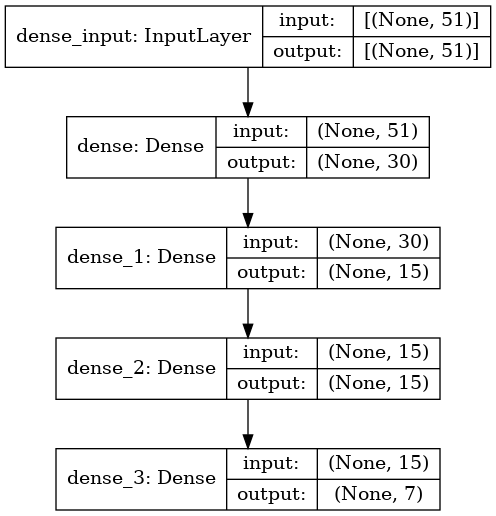
\includegraphics[width=0.7\textwidth]{./TeX_files/img/twohiddenmodel.png}
\caption{Two hidden layers model diagram.}
\label{fig:twohiddenmodel}
\end{figure}

\begin{figure}
\centering
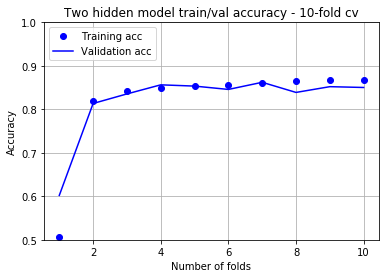
\includegraphics[width=0.7\textwidth]{./TeX_files/img/twohiddenmodelacc.png}
\caption{Two hidden layers model accuracy.}
\label{fig:twohiddenmodelacc}
\end{figure}

\begin{figure}
\centering
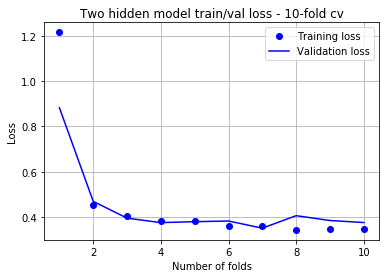
\includegraphics[width=0.7\textwidth]{./TeX_files/img/twohiddenmodelloss.png}
\caption{Two hidden layers model losses.}
\label{fig:twohiddenmodelloss}
\end{figure}

\begin{figure}
\centering
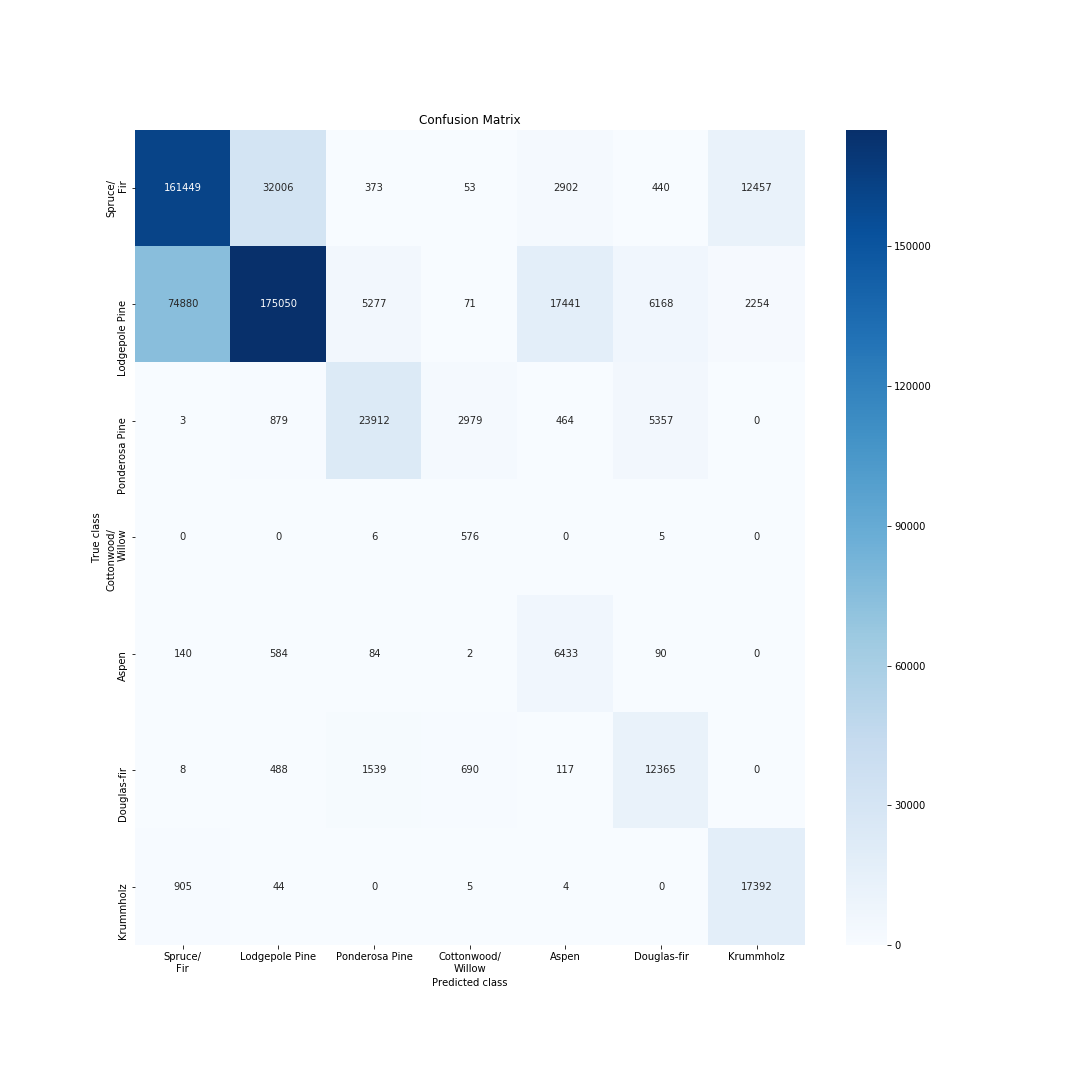
\includegraphics[width=\textwidth]{./TeX_files/img/twohiddenconfmatheatmap.png}
\caption{Heat-map rendering of the confusion matrix for the two hidden layers model.}
\label{fig:twohiddenconfmatheatmap}
\end{figure}

\begin{table}
\centering
\resizebox{0.9\textwidth}{!}{
\begin{tabular}{ccccc}
& precision & recall & f1-score & support     \\ \hline
Spruce/Fir        & 0.6801    & 0.7700 & 0.7223   & 209680 \\ \hline
Lodgepole Pine    & 0.8374    & 0.6226 & 0.7142   & 281141 \\ \hline
Ponderosa Pine    & 0.7666    & 0.7118 & 0.7382   & 33594  \\ \hline
Cottonwood/Willow & 0.1316    & 0.9813 & 0.2321   & 587    \\ \hline
Aspen             & 0.2351    & 0.8773 & 0.3708   & 7333   \\ \hline
Douglas-fir       & 0.5062    & 0.8131 & 0.6240   & 15207  \\ \hline
Krummholz         & 0.5418    & 0.9478 & 0.6894   & 18350  \\ \hline
weighted avg      & 0.7479    & 0.7019 & 0.7104   & 565892 \\ \hline
test set accuracy          & 0.7019    & 0.7019 & 0.7019   & 0.7019      \\ \hline
\end{tabular}
}
\caption{Precision, recall, f1-score summary table for the two hidden layers model.}
\label{tab:twohiddenclassificationrep}
\end{table}